\documentclass{beamer}


\usepackage{animate}
\usepackage[spanish]{babel}
\usepackage[utf8]{inputenc}
\usepackage{amsmath}
\usepackage{pgfplots}
 \usepackage{graphicx}
\usetheme{Madrid}
\title{Punto Fijo}

\author{H.D Salinas \\
Curso de métodos computacionales\\
Universidad de Antioquia\\}


\date{\today}

\begin{document}

\begin{frame}
  \titlepage
\end{frame}

% Diapositiva 1: Introducción al método
\begin{frame}{Introducción al método}

El método del punto fijo es un método iterativo que permite resolver ecuaciones no lineales de la forma $f(x)=0$, 
El método consiste en los siguientes pasos:
\begin{itemize}
    \item Definir $g(x)=x-f(x)$
    \item Definir $g(x_0)=x_0-f(x_0)=x_0$
    \item Definir el punto $p_0$, evaluar $g(p_0)$.
    \item Calcular el intercepto con la linea reacta $p_1=g(p_0)$  ,$(g(p_0), g(p_0))$


    \item Ir al punto $p_1=g(p_0)$
    $(g(p_0)),g(p_0)$

    \item el siguiente punto es $p_1$, $(p_1, g(p_1))$
    \item Comparar $p_1$ con $g(p_1)$, si la condiciones no se satisface, repetir desde el paso 2, pero no con $p_1$
\end{itemize}



\end{frame}



\begin{frame}{Interpretacion Geométrica}

\begin{figure} 
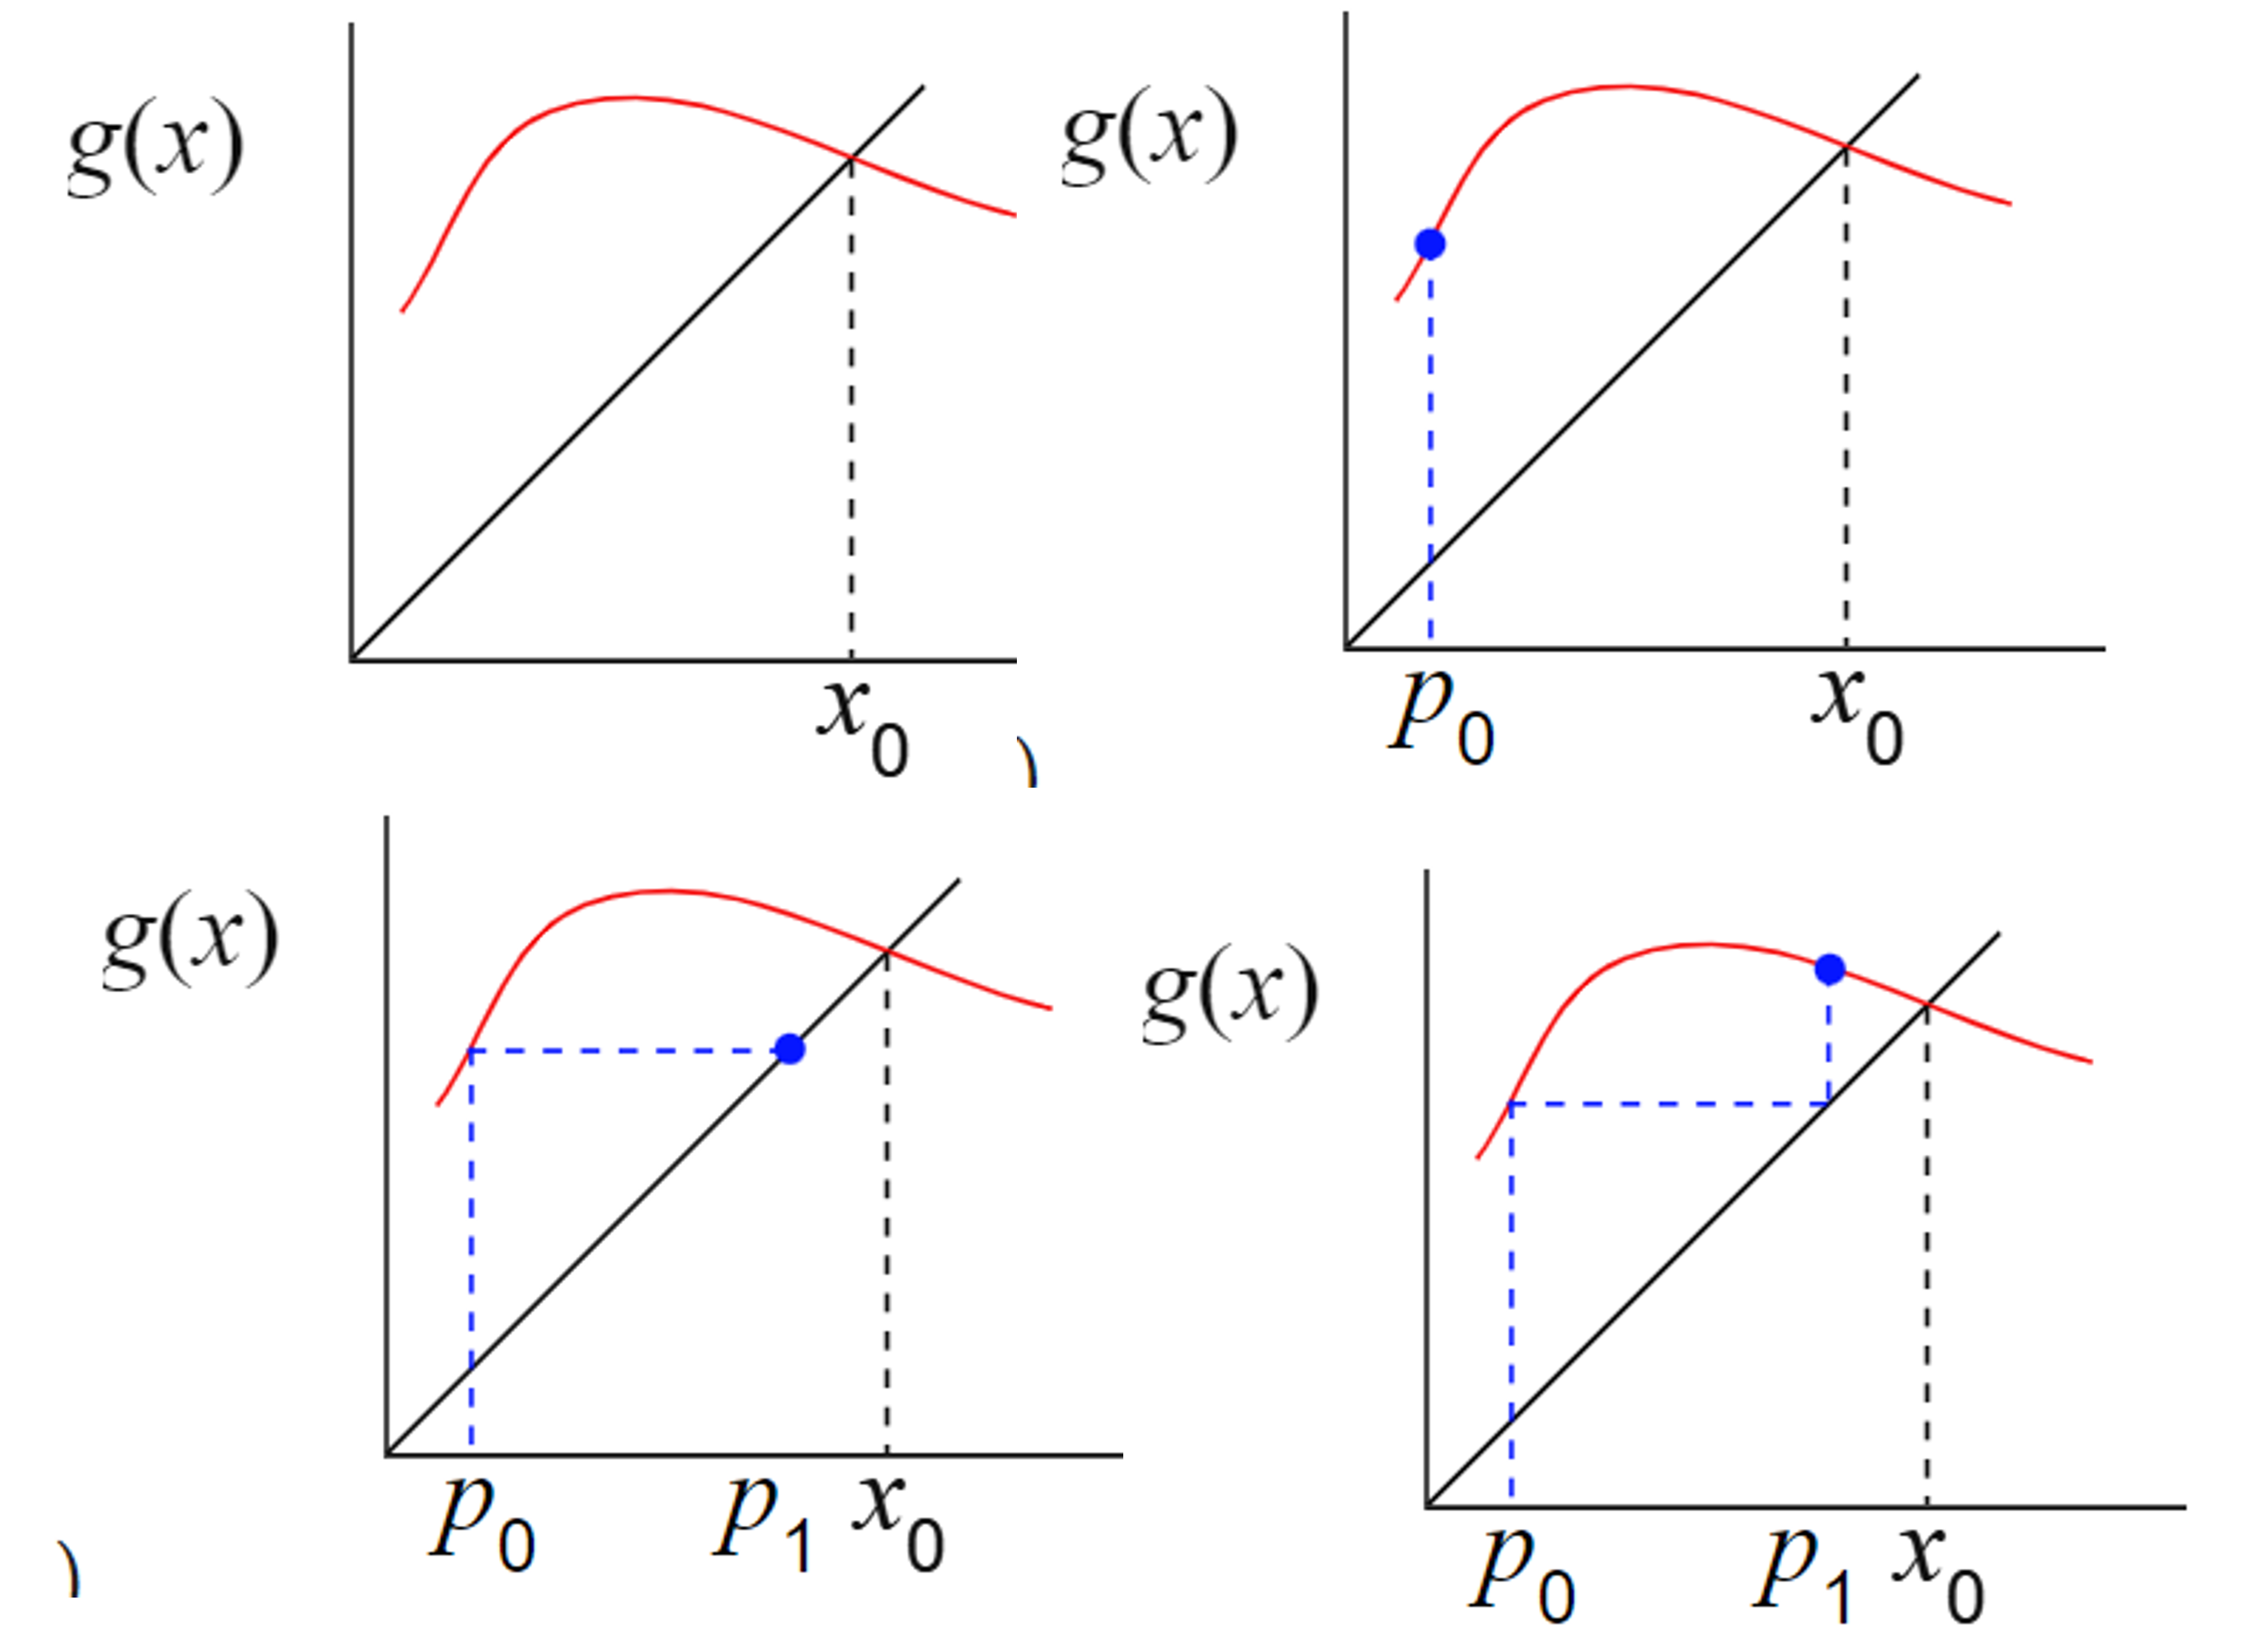
\includegraphics[width=0.7\textwidth]{puntoFijo.png} \caption{Interpretacion Gemétrica.} \end{figure} 
\end{frame}

\end{document}